% Elaborado por Marcelo Chávez | marcelo_chavez_ec@outlook.com | 0983332687
% LinkedIn: https://www.linkedin.com/in/marcelochavezec
\usepackage{tikz}
\usepackage{eso-pic}
\usepackage{fancyhdr}
\usepackage{fontawesome5}
\usepackage{etoolbox}
\usepackage{fvextra}
\usepackage{xurl}
\usepackage{microtype}
\definecolor{MSPAzul}{HTML}{003872}
\definecolor{MSPTurquesa}{HTML}{008A99}
\definecolor{Cuadricula}{HTML}{E4EDF4}
\definecolor{MargenCuaderno}{HTML}{E5B9B9}
\AddToShipoutPictureBG{%
  \begin{tikzpicture}[remember picture,overlay]
    \draw[step=5mm,Cuadricula,line width=0.12pt]
      (current page.south west) grid (current page.north east);
    \draw[MargenCuaderno,line width=0.35pt]
      ([xshift=16mm]current page.south west) -- ([xshift=16mm]current page.north west);
  \end{tikzpicture}}
\pagestyle{fancy}
\fancyhf{}
\fancyhead[L]{
\includegraphics[width=5.8cm]{recursos/logo_msp.png}}
\fancyhead[R]{
\includegraphics[width=1.8cm]{recursos/banco_mundial.png}}
\renewcommand{\headrulewidth}{0.35pt}
\renewcommand{\footrulewidth}{0.2pt}
\newcommand{\PieIzquierdo}{\parbox[b]{0.65\textwidth}{\raggedright\fontsize{6.6}{8.2}\selectfont
  \AutorManual\\[2pt]\CargoManual\\[2pt]\ContactoManual}}
\newcommand{\PieDerecho}{\parbox[b]{0.33\textwidth}{\raggedleft\fontsize{6.6}{8.2}\selectfont
  Manual de la API de integración\\[2pt]-- página \thepage}}
\fancyfoot[L]{\PieIzquierdo}
\fancyfoot[R]{\PieDerecho}
\fancypagestyle{plain}{\fancyhf{}
  \fancyhead[L]{
\includegraphics[width=5.8cm]{recursos/logo_msp.png}}
  \fancyhead[R]{
\includegraphics[width=1.8cm]{recursos/banco_mundial.png}}
  \fancyfoot[L]{\PieIzquierdo}\fancyfoot[R]{\PieDerecho}}
% La portada no se cuenta; la tabla de contenidos inicia en la página 1.
\pretocmd{\tableofcontents}{\clearpage\pagenumbering{arabic}\setcounter{page}{1}}{}{}
\setkomafont{chapter}{\normalfont\LARGE\bfseries\color{MSPAzul}}
\setkomafont{section}{\normalfont\large\bfseries\color{MSPAzul}}
\setkomafont{subsection}{\normalfont\normalsize\bfseries\color{MSPAzul}}
\RedeclareSectionCommand[beforeskip=12pt,afterskip=14pt]{chapter}
\DefineVerbatimEnvironment{Highlighting}{Verbatim}{commandchars=\\\{\},breaklines=true,breakanywhere=true,breaknonspaceingroup=true,fontsize=\footnotesize}
\fvset{fontsize=\footnotesize,breaklines=true,breakanywhere=true,breaknonspaceingroup=true}
\setlength{\emergencystretch}{3em}
\setlength{\parskip}{4pt}
\renewcommand{\maketitle}{%
  \hypersetup{pageanchor=false}\begin{titlepage}\thispagestyle{empty}\thispdfpagelabel{Portada}
  \noindent
\includegraphics[width=6.8cm]{recursos/logo_msp.png}\hfill
  
\includegraphics[width=2.0cm]{recursos/banco_mundial.png}\par
  \vspace*{26mm}
  \begin{center}
  {\color{MSPAzul}\fontsize{30}{35}\selectfont\bfseries Manual de la API de integración\par}
  \vspace{7mm}
  {\color{MSPAzul}\fontsize{22}{28}\selectfont\bfseries Módulo de Indicadores de Presidencia\par}
  \vspace{9mm}
  {\color{MSPTurquesa}\large Tecnología: Python · FastAPI · R Shiny · Nginx\par}
  \vspace{5mm}
  {\normalsize Construcción, instalación, configuración, publicación, consumo y pruebas.\par}
  \vspace{18mm}
  {\large \textbf{Elaborado por:} \AutorManual\par}
  \vspace{2mm}
  {\normalsize\CargoManual\par}
  \vspace{6mm}
  {\small\href{mailto:marcelo_chavez_ec@outlook.com}{\faEnvelope\enspace\CorreoManual}\par}
  \vspace{2mm}
  {\small\href{tel:+593983332687}{\faIcon{mobile-alt}\enspace\MovilManual}\quad
    \href{https://www.linkedin.com/in/marcelochavezec}{\faLinkedin}\par}
  \vfill
  \end{center}
  {\raggedright\fontsize{7}{9}\selectfont \textbf{Versión documental:} 22 de octubre de 2026\par}
  \end{titlepage}\hypersetup{pageanchor=true}}
